
\section{Multi-Agent Systems}


\subsection{Agents and Environments in Artificial Intelligence}

\begin{figure}
\begin{centering}
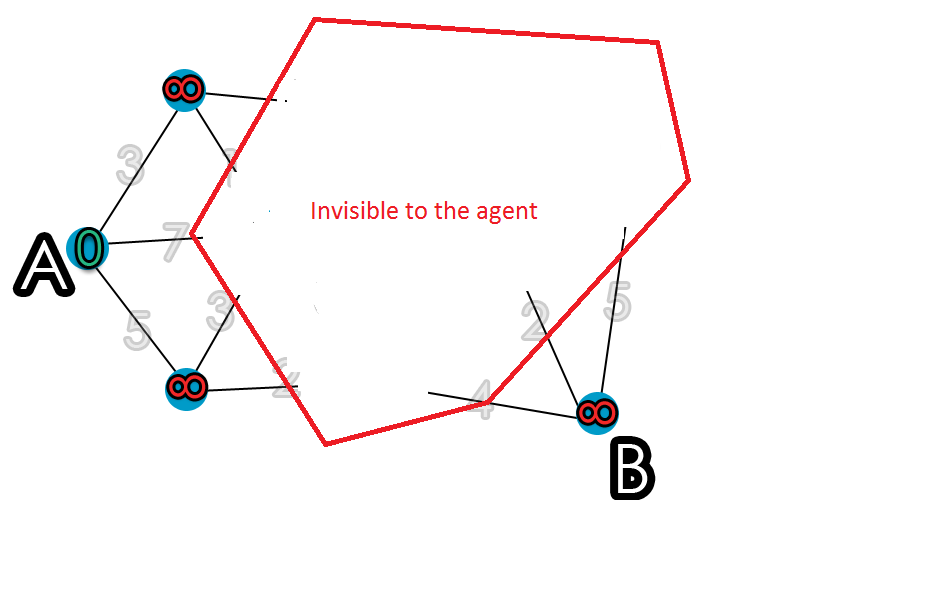
\includegraphics[width=0.5\textwidth,bb = 0 0 200 100, draft, type=eps]{MASNodeSearch.png}
\par\end{centering}

\caption{What an agent can see of a graph where it tries to move from node
A to node B.\label{fig:MASNodeSearch}}


\end{figure}


In artificial intelligence, an agent is something that can perform
actions in and (partially or fully) perceive the state of the environment
it is situated in. As an example, consider an agent tasked with finding
the shortest route between two nodes in a weighted, undirected graph,
with the limitation that it can only see the nodes that have an edge
to the one it is standing in, an example of the graph can be seen
on fig. \ref{fig:MASNodeSearch}. We will now use this example to
describe what (Russel, Norvig, 2010) calls a \emph{task environment},
consisting of definitions for the performance measure for the agent,
the environment it acts in, the actions it can take, and its facilities
for perception:
\begin{description}
\item [{Environment}] The environment is a model of the world the agent
acts in. In our example, it is described as a graph. The environment
may also contain artifacts for agents to interact with, such as a
packages to pick up or obstacles to navigate around.
\item [{Actions}] This denotes what actions the agent can take to change
the state of the environment or itself. In the example, the agent
would have a \emph{move} action, allowing it to move to an adjacent,
connected node.
\item [{Percepts}] If the agent is to make intelligent decisions, it must
be able to perceive the current state of the world -- that is, itself
and the environment. Such a fragment of information that the agent
have sensed is called a percept. In the running example, the agent
can perceive the nodes immediately connected to the one it is standing
on, as well as the edges to those nodes.
\item [{Performance}] For an agent to be as efficient as possible, it is
useful to have a performance measure describing how well the agent
is executing the task at hand. In the provided example, the performance
measure could be defined in terms of the number of actions taken per
unique node visited, giving the agent an idea of the amount of redundancy
in its pathfinding.
\end{description}
While the task environment can be used to succinctly describe the
properties of the world, it says nothing of the logic that the agent
applies to perform tasks in the world. This is left in the hands of
an \emph{agent program}, which is responsible for processing the percepts
and choosing actions for an agent. In general, an agent program receives
percepts and chooses an appropriate action based on the knowledge
available to it in an aptly named \emph{percept-action} \emph{cycle}.
This knowledge may just be the current percepts, or it may be all
the percepts retreived so far. When choosing an action, it may take
into consideration how different actions would affect the world, and
how much closer performing the action would bring the agent to its
goal. Agents with such capable agent programs are called \emph{utility-based
agents} in (Russel, Norvig, 2010).


\subsection{Multi-Agent Systems}

While there is no strict, universal definition of what constitutes
a multi-agent system, the following seems to represents the simplest
consensus: \emph{In a multi-agent system, several intelligent agents
act and interact more or less autonomously in an environment}. The
interacting of agents may be of any character, the important part
is that each agent can be aware of the others and affect their execution
directly or indirectly. Here, a direct effect means changing another
agents state, eg.\ by moving it into another postition or decreasing
its health. An indirect effect could be communicating with the agent,
suggesting another execution path. For instance, a system in which
agents compete for ressources and hinder other agents' progress is
a multi-agent system, as is a system in which the agents work together
towards a common goal. 

While the former may be useful in simulating certain systems, the
latter is more interesting in software design, as such an approach
could conceivably lead to more decentralized problem solving. A mixture
of the two approaches can also be used, as in the Multi-Agent Programming
Contest\texttt{\emph{}}%
\footnote{\texttt{multiagentcontest.org}%
}, where teams of cooperating agents compete for points. In this case,
the goal for each team is to develop the best strategy, where performance
is measured by competitiveness.

In addition to the above, limiting the agents' knowledge of the state
of the world is a desirable characteristic of a MAS; otherwise, there
would be no need for the agents to communicate, and they could just
as well be subroutines of a single agent (Panait and Luke, 2005).
It could still be modelled as a MAS, of course, but not a very interisting
one. Additionally, the case could be made that the less agents know
of the world, the less information they have to process when searching
for an action to execute, thus reducing their computational load.
On the other hand, less information can cause the agent to follow
a suboptimal execution path, causing a trade-off between computation
time and optimality. 

One of the strong points of multi-agent systems is that it consists
of several pieces of software running more or less autonomously. As
mentioned above, this allows for developing decentralized systems,
where agent programs runs on different threads or servers. In the
context of distributed systems, less dependency on a central intelligence
is of course preferred. 

Furthermore, MASs are useful when simulating naturally occuring systems
wherein several ``agents'' interact with each other An example of
this could be a group of animals around a watering hole, where some
are prey and some are predators.


\subsection{The GOAL Agent Programming Language}

In this section we will outline the GOAL language based on ~\cite{Hindriks06}.

Several APLs (Agent Programming Languages) have been developed to
suit the defining characters of agents and their interaction with
environments as we have described them above. In this section, we
will focus on the relatively new GOAL APL, which can be written using
the prolog logic programming language.

In GOAL, code is segmented into sections describing:
\begin{itemize}
\item What it knows
\item What it wants to achieve
\item What it can do
\item How it handles new information (percepts) from the environment
\item The actual logic for choosing an appropriate action to execute
\end{itemize}
The first two points in the list will be explained below. 


\subsubsection*{Mental State}

GOAL provides the notion of \emph{mental state} of an agent, which
describes what the agent knows and what it aims to achieve. Specifically,
it consists of the following three components:
\begin{description}
\item [{Knowledge}] describes what the engine knows to be universally true.
This information is completely static; it is something the agent is
``born'' with, and can not be changed. In other words, this describes
the rules and constants of the system.
\item [{Beliefs}] are facts the agent deduces during its execution, using
its knowledge. Beliefs can be updated at runtime by using the \texttt{insert($\varphi$)}
and \texttt{delete($\varphi$)} commands, where\texttt{ $\varphi$}
is a belief. The \texttt{bel($\varphi$)} operation can be used to
ascertain whether the agent believes that $\varphi$ holds.
\item [{Goals}] are what the agent strives to accomplish. These can be
dynamically updated along the way to acommodate for a changing world.
This is done with the \texttt{adopt($\varphi$)} and \texttt{drop($\varphi$)}
commands, where $\varphi$ is a goal. \texttt{goal($\varphi$)} checks
whether $\varphi$ is currently a goal of the agent. If a goal have
been achieved -- that is, if the agent's current beliefs and knowledge
satifies a goal -- it is automatically removed from the \texttt{goals}
collection, as the agent would otherwise keep trying to accomplish
it. 
\end{description}
The information in the mental state is stored as logical statements
in prolog. The operations mentioned above for querying and modifying
the mental state thus takes a prolog statement as input.


\subsubsection*{Acting and Perceiving}

When a GOAL program is run, it executes the following steps, in order:
\begin{enumerate}
\item Receive percepts
\item Update the goals and beliefs of the agent if needed
\item Choose an appropriate action to execute
\end{enumerate}
This is repeated in a cycle. 

The processing of new percepts mentioned in point \#2 is handled in
the \texttt{event module} of the agent program. Here, all new percepts
in the current cycle can be inspected, and the mental state of the
agent can be updated. If, for example, the agent perceives that it
is in a different location than in the previous cycle, this module
can be used to change its beliefs accordingly. If the world have changed
drastically, the agent may also choose to drop goals that can no longer
be achieved, and/or adopt goals that seems more fruitful to pursue.
As such, the processing of percepts is the primary place to change
the mental state of the agent.

The choosing of an action is where the agent decides -- based on its
mental state -- which execution path it should take. The actions themselves
are provided in an \texttt{action specification} section of the program,
where each action denotes pre- and postconditions of the action. That
is, what must hold for the action to be executed and what effect it
will have on the environment. An action is not considered for execution
if its precondition does not hold. If it does hold and the action
is taken, the logical statements in the postcondition is inserted
into the belief base. 

When an action have been chosen in GOAL, it is only \emph{set} to
be executed, that is, GOAL requests that it be executed. It might
be that the program managing the agent in the environment sees fit
to not execute it, or that the action fails (if the agent tries to
move into a wall, for example). In that case, GOAL only knows about
the failure of the action if it is somehow obvious from the next set
of percepts it receives. In light of this, postconditions on actions
should only be used when it absolutely certain that what the postcondition
specifies is true, as it may otherwise insert flawed information into
the agents beliefs.


\subsection{The Environment Interface Standard}

Several agent programming languages -- including GOAL -- is only concerned
with the agent logic of a MAS. To provide a world in which these agents
can function, they need to be connected to a program providing an
environment. 

EIS (Environment Interface Standard) \texttt{\emph{{[}Reference EIS
technical report{]}}} is a Java framework, which can be used to design
environments and connect them to agent programming languages. As such,
it does not assume much about the implementation of the environments
or the agents inhabiting it. 

It provides \texttt{entities} which can function as the bodies of
agent programs, and means for receiveing commands and returning percepts
to the connected agents.When using EIS, the environment designer can
handle actions sent by the agent programs with the \texttt{performAction}
method to define exactly how they affect the world the designer have
constructed. Percepts can be requested explicitly through the \texttt{getAllPercepts}
method (this is how GOAL gets its percepts from EIS) or as notifications,
for APLs that support it. 

The main point of EIS is to provide a standard (hence the name) for
developing MASs, such that environments designed with this standard
can easily be interfaced with different APLs. As such, EIS comes pre-loaded
with bindings for several common APLs such as GOAL and Jason. As part
of this standard, the IILang (Interface Immediate Language) abstract
syntax tree have been developed. It can be used to easily and unambiguously
define actions and percepts consisting of identifiers, numerals, representations
of functions over identifiers and numerals, and lists of identifiers,
numerals and functions. These IILang objects can be created as native
Java objects and easily parsed to -- in the case of GOAL -- prolog
statements, and vice versa.

In conclusion, it is important to note that GOAL and EIS are supposed
to be two components of a multi-agent system. GOAL is not supposed
to maintain an environment, and EIS is not very well suited for implementing
agent logic.


\subsubsection*{References}

Stuart J. Russel, Peter Norvig, ``Artificial Intelligence: A Modern
Approach'', Prentice Hall, Upper Saddle River, New Jersey 07458,
3rd ed., 2010\\


Panait, Luke, ``Cooperative Multi-Agent Learning: The State of the
Art'', Autonomous Agents and Multi-Agent Systems, Volume 11, Issue
3, pp.\ 387-434, 2005.
